\documentclass{pjatk}

\usepackage{tocloft}
\usepackage{hyperref}
\usepackage[english,polish]{babel}
\usepackage{tikz-uml}
\usepackage[acronym, toc]{glossaries}

\addbibresource{attachments/bibliography.bip}

\makeglossaries
%! Author = Mateusz Budzisz
%! Date = 08/11/2023

\newglossaryentry{pwa}{name={Progressive Web App},
description={Progressive Web App (PWA) to progresywna aplikacja internetowa uruchamiana tak jak zwykła strona internetowa,
 ale umożliwiająca stworzenie wrażenia działania jak natywna aplikacja mobilna lub aplikacja desktopowa. }
}
\newglossaryentry{aws}{name={Amazon Web Services},
description={Amazon Web Services (AWS) – pakiet usług chmurowych oferowanych przez Amazon},
}
\newglossaryentry{gcp}{name={Google Cloud Platform},
description={Oferowany przez Google zestaw usług chmurowych, obejmuje szereg modułowych usług chmurowych, w tym przetwarzanie danych, przechowywanie danych, analitykę danych oraz uczenie maszynowe, a także zestaw narzędzi zarządzania.}
}
\newglossaryentry{azure}{ name={Azure},
description={Microsoft Azure to platforma chmurowa firmy Microsoft stworzona w modelu PaaS (Platform as a Service)}
}
\newglossaryentry{osm}{name={Open Street Map},
description={OpenStreetMap (OSM) – projekt społeczności internetowej mający na celu stworzenie darmowej, swobodnie dostępnej mapy całej kuli ziemskiej.}}
\newglossaryentry{lsp}{name={Language Service Protocol},
description={Protokół Language Server Protocol (LSP) to otwarty protokół oparty na JSON-RPC, stosowany pomiędzy edytorami kodu źródłowego lub zintegrowanymi środowiskami programistycznymi (IDE) a serwerami, które dostarczają "narzędzia inteligencji językowej": specyficzne dla języków programowania funkcje, takie jak uzupełnianie kodu, podświetlanie składni oraz oznaczanie ostrzeżeń i błędów, a także rutyny refaktoryzacji.}
}
\newglossaryentry{osw}{
name={Open Weather Map},
description={Open Weather Ma} 
}
\newglossaryentry{http}{name={Hyper Text Transfer Protocol},
description={ Hyper Text Transfer Protocol protokół stworzony przez Tima Bernersa-Lee na potrzeby komunikacji między klientem a serwerem w sieci WWW (ang. World Wide Web).}
}

\newglossaryentry{drag-n-drop}
{
    name={Drag and drop},
    description={Technologia umożliwiająca interfejsom użytkownika w przeglądarkach internetowych korzystanie z funkcji przeciągania i upuszczania elementów. Użytkownik może wybrać elementy do przeciągania za pomocą myszy, przeciągnąć te elementy do elementu docelowego i upuścić je, zwalniając przycisk myszy. Podczas operacji przeciągania półprzezroczysta reprezentacja przeciąganych elementów podąża za wskaźnikiem myszy.}
}

\newglossaryentry{on-demand}
{
    name={On-demand},
    description={Rodzaj oprogramowania charakteryzującego się dynamicznym czasem pracy, uruchamiane na rządanie, gdy poda wynik program kończy pracę zamiast oczekiwać następnego zapytania}
}

\newglossaryentry{refactoring}
{
    name={Refactoring},
    description={Znaczna zmiana konstrukcji programu mająca na celu usprawnienie oprogramowania bądź dostosowanie go do nowych wymogów}
}

\newglossaryentry{ui}
{
    name={UI},
    description={Interfejs użytkownika}
}

\newglossaryentry{frontend}
{
    name={Frontend},
    description={Oprogramowanie składające się z UI z którym docelowy użytkownik będzę wchodził w interakcję}
}

\newglossaryentry{backend}
{
    name={Backend},
    description={Oprogramowanie pozbawione UI z którym docelowy użytkownik będzę wchodził w interakcję, potrzebne do prawidłowej pracy Frontendu}
}

\newglossaryentry{job}
{
    name={Job},
    description={Oprogramowanie, które ma z góry określony cel, po jego uruchomieniu natychmiast zaczyna je wykonywać, nie wchodzi w interakcje z użytkownikiem docelowym, po zakończeniu kończy swoje życie}
}


\newglossaryentry{rendering}
{
    name={Wyrenderowanie},
    description={Stworzenie UI z postaci kodu do postaci konsumowalnej przez użytkownika docelowego}
}

\newglossaryentry{hello-world}
{
    name={Hello world},
    description={Minimalny reprezentatywny program w danej technologii}
}

\newglossaryentry{hermetyzacja}
{
    name={Hermetyzacja},
    description={Hermetyzacja opgorgramowania określa dobrą praktykę programistyczną polegającą na izolacji komponentów w aplikacji tak aby o sobie nie wiedziały gdy nie muszą o sobie wiedzieć}
}

\newglossaryentry{infra-as-code}
{
    name={Infrastructure as a code},
    description={Sposób opisania architektury systemu poprzez napisanie programu tworzącego docelową architekturę przy pomocy abstrakcji dostarczonych przez dostawcę mocy obliczeniowej}
}

\newglossaryentry{on-prem}
{
    name={On-premise},
    description={Oprogramowanie hostowane na samodzielnie zarządzanej infrastrukturze}
}

\newglossaryentry{virt}
{
    name={Wirtualizacja},
    description={Podział serwera na maszyny o mniejszej mocy obliczeniowej, aby umożliwić podział podzespołów pomiędzy klientów tak, aby nic o sobie nawzajem nie wiedzieli}
}

\newglossaryentry{arm}
{
    name={Architektura ARM},
    description={Architektura silnej ręki lol}
}
\newglossaryentry{poidef}
{
    name={POI},
    description={Point of interest (w skrócie POI) to punkt w przestrzeni, najczęściej na powierzchni Ziemi.}
}
\newglossaryentry{openlayers}
{
    name={Openlayers},
    description={OpenLayers to biblioteka napisana w języku JavaScript, ułatwiająca dodawanie dynamicznych map na stronach internetowych.}
}
\newglossaryentry{reflink}
{
    name={Reflink},
    description={Reflink to specjalny link, który zawiera unikalny kod identyfikacyjny, pozwalający na monitorowanie ruchu i przekierowań z innych źródeł.}
}
\newglossaryentry{sla}
{
    name={SLA},
    description={Service Level Agreement, SLA (umowa o gwarantowanym poziomie świadczenia usług) to umowa utrzymania i systematycznego poprawiania ustalonego między usługodawcą a usługobiorcą poziomu jakości usług poprzez stały cykl obejmując: uzgodnienia,
    monitorowanie usługi, raportowanie, przegląd osiąganych wyników.}
}
\newglossaryentry{sws}
{
    name={SWS},
    description={Specyfikacja Wymagań Systemowych }
}
\newglossaryentry{moscow}
{
    name={MoSCoW},
    description={Metoda MoSCoW to technika priorytetyzacji wykorzystywana w analizie biznesowej i przy tworzeniu oprogramowania w celu osiągnięcia wspólnego zrozumienia pomiędzy interesariuszami co do znaczenia, jakie ma dla nich dostarczenie każdego z wymagań. Inne nazwy metody to priorytetyzacja MoSCoW lub analiza MoSCoW.}
}
\newglossaryentry{CRUD}
{
    name={CRUD},
    description={CRUD (od angielskiego create, read, update, delete, tłumaczenie utwórz, odczytaj, aktualizuj, usuń) – cztery podstawowe funkcje w aplikacjach korzystających z bazy danych, które umożliwiają zarządzanie nią.}
}
\newglossaryentry{stadiamaps}
{
    name={Stadia Maps},
    description={Stadia Maps oferuje komercyjne interfejsy API do mapowania i wyznaczania tras, głównie oparte na OpenStreetMap.}
}

\newglossaryentry{mevo}
{
    name={Mevo},
    description={Mevo to system bezobsługowych wypożyczalni rowerów miejskich.}
}
\newglossaryentry{scraping}
{
    name={Web scraping},
    description={Data scraping to technika ekstrakcji danych z witryn internetowych.}
}
\newglossaryentry{lighthouse}
{
    name={Lighthouse},
description={Lighthouse to narzędzie open-source stworzone przez Google do automatycznego audytu stron internetowych. Analizuje wydajność, dostępność, zgodność z progresywnymi aplikacjami webowymi (PWA), SEO i najlepszymi praktykami. Wyniki audytów pomagają poprawić jakość i funkcjonalność stron internetowych. Narzędzie można uruchomić z poziomu Chrome DevTools, jako rozszerzenie Chrome lub z wiersza poleceń.}
}
\newglossaryentry{openmeteo}
{
    name={OpenMeteo},
description={OpenMeteo to darmowa, otwarta usługa dostarczająca prognozy pogody poprzez interfejs API. Oferuje precyzyjne prognozy dla różnych lokalizacji na świecie, umożliwiając integrację z aplikacjami i serwisami internetowymi.}
}


\studfield{Informatyka}
\studtype{Zaoczne}
\title{Planer Mapy Miejskiej}
\engtitle{City Map Planner}
\acronym{City Planner}
\titledate{2023-10-14}
\supervisor{prof. dr hab. Marek A. Bednarczyk}
\author{Mateusz Budzisz}{s24048}{Aplikacje Internetowe}{Zaoczny}
\author{Wiktor Rostkowski}{s23141}{Aplikacje Internetowe}{Zaoczny}
\author{Sebastian Kreft}{s23133}{Aplikacje Internetowe}{Zaoczny}
\author{Damian Kreft}{s23447}{Aplikacje Internetowe}{Zaoczny}
\consultant{--- brak ---} % Koniecznie trzeba podać brak, albo wpisać konsultantów tak jak przy autorach
\projectgoals{Stworzenie interaktywnej mapy miejskiej do planowania zwiedzania atrakcji turstycznych z wkykorzystaniem dynamicznych danych}
\productsandservices{Aplikacja progresywana}
\mainfunctionalities{Planowanie trasy}
\successmeasure{Wdrożenie rozwiązania jako oficjalnego rozwiązania miejskiego}
\projlimitations{Brak budżetu}
\date{\today}
\nabstract{
	Praca zakłada utworzenie interaktywnej mapy z punktami zainteresowań na podstawie listy atrakcji turystycznych wyróżnionych przez urząd miejski,
	umożliwiającej kompleksowe zaplanowanie optymalnej trasy zwiedzania z uwzględnieniem środków komunikacji miejskiej,
	godzin otwarcia atrakcji turystycznych oraz warunków pogodowych.
}

\graphicspath {{attachments/}}

\begin{document}

	% PJATK Template begin
	\maketitle
	\makeprojectcard
	\makedeclaration
	% PJATK Template End

	\tableofcontents
	\clearpage
	%! Author = Wiktor Rostkowski
%! Date = 29/04/2024

\chapter{Testy}
\label{ch:testy}

%! Author = Wiktor Rostkowski, Mateusz Budzisz
%! Date = 29/04/2024

\chapter{Testy}
\label{ch:testy}

\section{Testy jednostkowe}
\label{sec:testy-jednostkowe}
W ramach projektu potok frontend wykonał 151 testów. \newline
W ramach projektu potok backend wykonał 159 testów. \newline
W ramach projektu potok dokumentacja wykonał 328 testów. \newline

\section{Testy wydajnościowe}
\label{sec:testy-wydajnosciowe}
Lighthouse
\section{Testy funkcjonalne}
\label{sec:testy-funkcjonalne}

\begin{figure}[H]
    \centering
    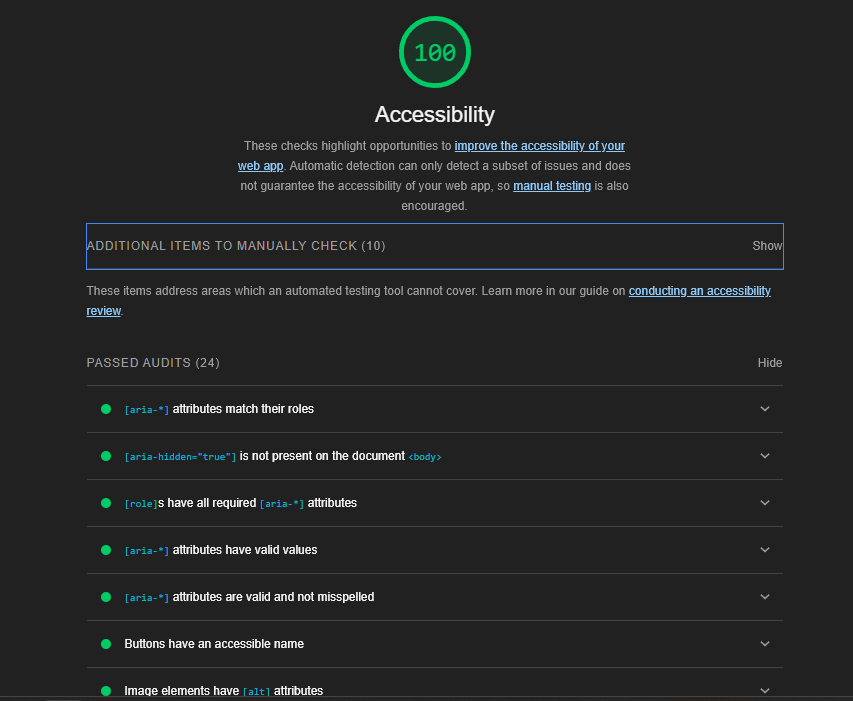
\includegraphics[width=1\textwidth]{attachments/testy-dostepnosci}
    \caption{Widok testu dostępności dla naszej aplikacji}
    \label{fig:testy-dostepnosci}
    \end{figure}


	%! Author = Wiktor Rostkowski
%! Date = 29/04/2024

\chapter{Testy}
\label{ch:testy}

%! Author = Wiktor Rostkowski, Mateusz Budzisz
%! Date = 29/04/2024

\chapter{Testy}
\label{ch:testy}

\section{Testy jednostkowe}
\label{sec:testy-jednostkowe}
W ramach projektu potok frontend wykonał 151 testów. \newline
W ramach projektu potok backend wykonał 159 testów. \newline
W ramach projektu potok dokumentacja wykonał 328 testów. \newline

\section{Testy wydajnościowe}
\label{sec:testy-wydajnosciowe}
Lighthouse
\section{Testy funkcjonalne}
\label{sec:testy-funkcjonalne}

\begin{figure}[H]
    \centering
    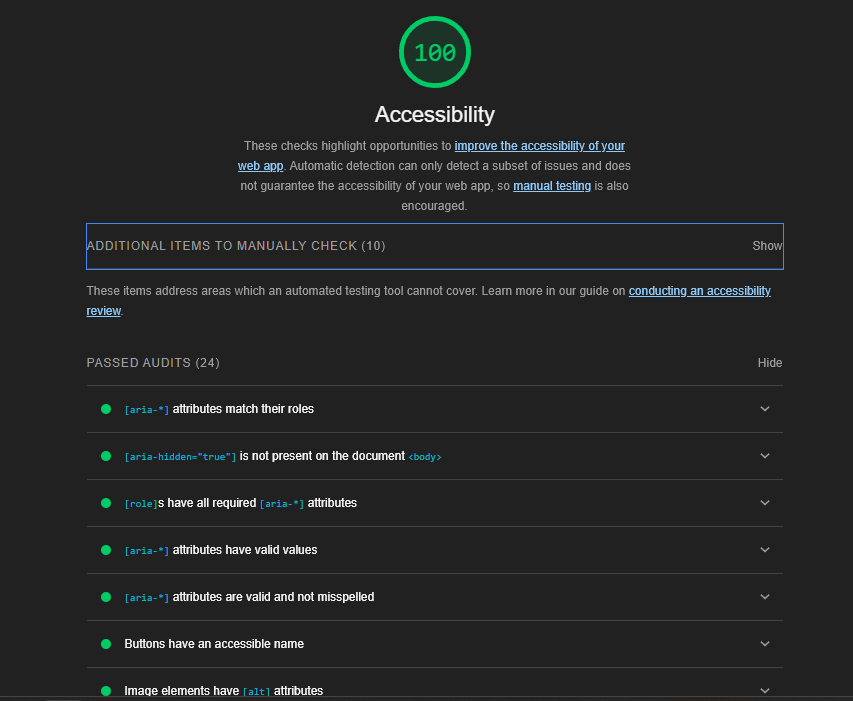
\includegraphics[width=1\textwidth]{attachments/testy-dostepnosci}
    \caption{Widok testu dostępności dla naszej aplikacji}
    \label{fig:testy-dostepnosci}
    \end{figure}


	%! Author = Wiktor Rostkowski
%! Date = 29/04/2024

\chapter{Testy}
\label{ch:testy}

%! Author = Wiktor Rostkowski, Mateusz Budzisz
%! Date = 29/04/2024

\chapter{Testy}
\label{ch:testy}

\section{Testy jednostkowe}
\label{sec:testy-jednostkowe}
W ramach projektu potok frontend wykonał 151 testów. \newline
W ramach projektu potok backend wykonał 159 testów. \newline
W ramach projektu potok dokumentacja wykonał 328 testów. \newline

\section{Testy wydajnościowe}
\label{sec:testy-wydajnosciowe}
Lighthouse
\section{Testy funkcjonalne}
\label{sec:testy-funkcjonalne}

\begin{figure}[H]
    \centering
    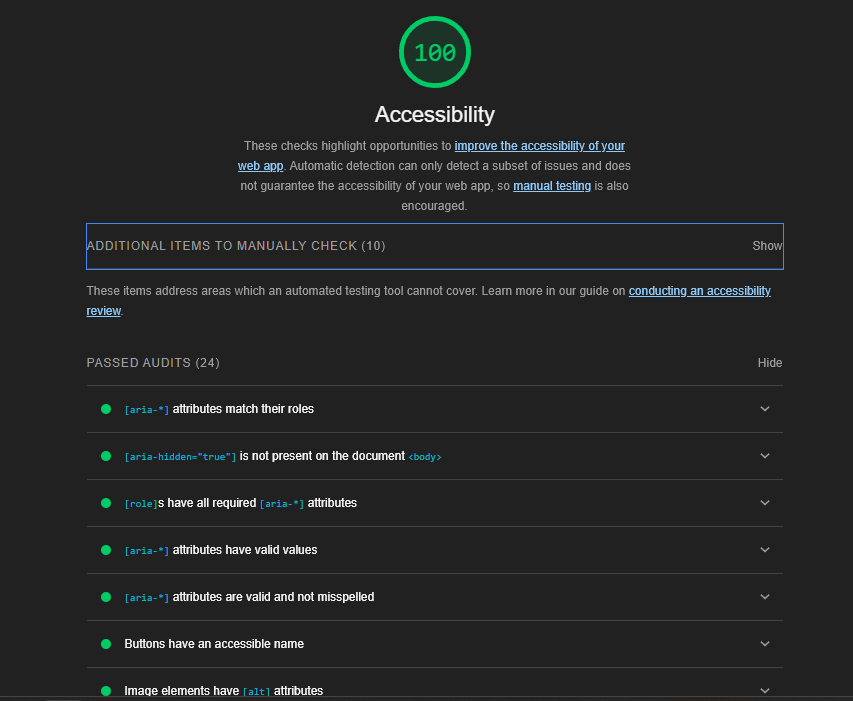
\includegraphics[width=1\textwidth]{attachments/testy-dostepnosci}
    \caption{Widok testu dostępności dla naszej aplikacji}
    \label{fig:testy-dostepnosci}
    \end{figure}


	%! Author = Wiktor Rostkowski
%! Date = 29/04/2024

\chapter{Testy}
\label{ch:testy}

%! Author = Wiktor Rostkowski, Mateusz Budzisz
%! Date = 29/04/2024

\chapter{Testy}
\label{ch:testy}

\section{Testy jednostkowe}
\label{sec:testy-jednostkowe}
W ramach projektu potok frontend wykonał 151 testów. \newline
W ramach projektu potok backend wykonał 159 testów. \newline
W ramach projektu potok dokumentacja wykonał 328 testów. \newline

\section{Testy wydajnościowe}
\label{sec:testy-wydajnosciowe}
Lighthouse
\section{Testy funkcjonalne}
\label{sec:testy-funkcjonalne}

\begin{figure}[H]
    \centering
    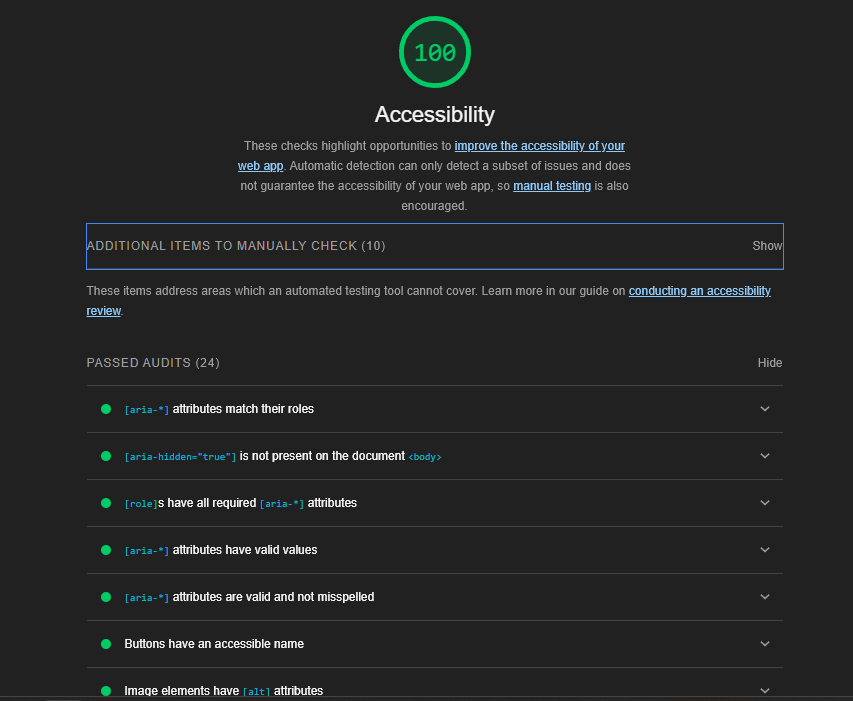
\includegraphics[width=1\textwidth]{attachments/testy-dostepnosci}
    \caption{Widok testu dostępności dla naszej aplikacji}
    \label{fig:testy-dostepnosci}
    \end{figure}


	%! Author = Wiktor Rostkowski
%! Date = 29/04/2024

\chapter{Testy}
\label{ch:testy}

%! Author = Wiktor Rostkowski, Mateusz Budzisz
%! Date = 29/04/2024

\chapter{Testy}
\label{ch:testy}

\section{Testy jednostkowe}
\label{sec:testy-jednostkowe}
W ramach projektu potok frontend wykonał 151 testów. \newline
W ramach projektu potok backend wykonał 159 testów. \newline
W ramach projektu potok dokumentacja wykonał 328 testów. \newline

\section{Testy wydajnościowe}
\label{sec:testy-wydajnosciowe}
Lighthouse
\section{Testy funkcjonalne}
\label{sec:testy-funkcjonalne}

\begin{figure}[H]
    \centering
    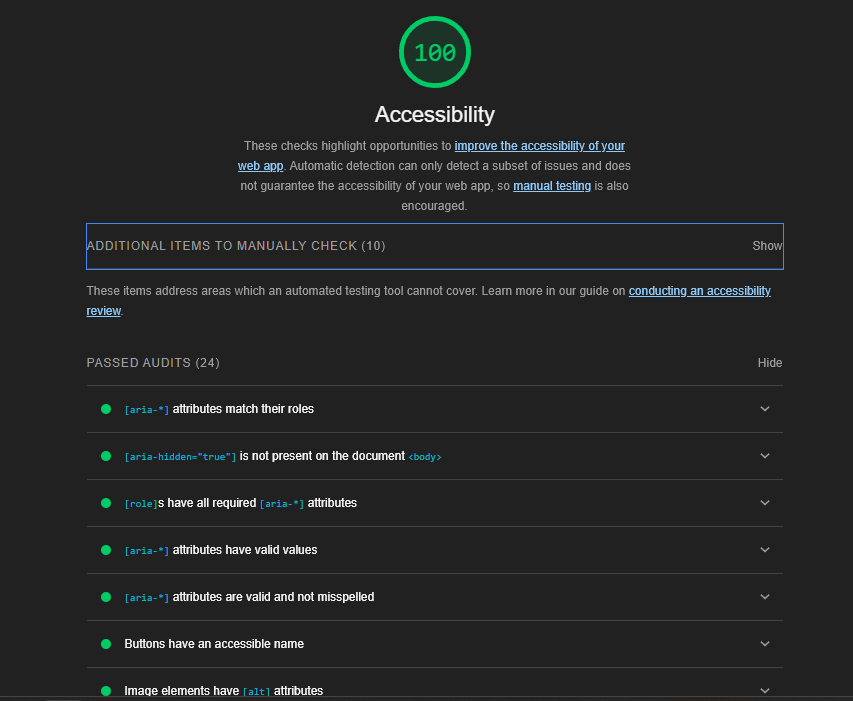
\includegraphics[width=1\textwidth]{attachments/testy-dostepnosci}
    \caption{Widok testu dostępności dla naszej aplikacji}
    \label{fig:testy-dostepnosci}
    \end{figure}


	%! Author = Wiktor Rostkowski
%! Date = 29/04/2024

\chapter{Testy}
\label{ch:testy}

%! Author = Wiktor Rostkowski, Mateusz Budzisz
%! Date = 29/04/2024

\chapter{Testy}
\label{ch:testy}

\section{Testy jednostkowe}
\label{sec:testy-jednostkowe}
W ramach projektu potok frontend wykonał 151 testów. \newline
W ramach projektu potok backend wykonał 159 testów. \newline
W ramach projektu potok dokumentacja wykonał 328 testów. \newline

\section{Testy wydajnościowe}
\label{sec:testy-wydajnosciowe}
Lighthouse
\section{Testy funkcjonalne}
\label{sec:testy-funkcjonalne}

\begin{figure}[H]
    \centering
    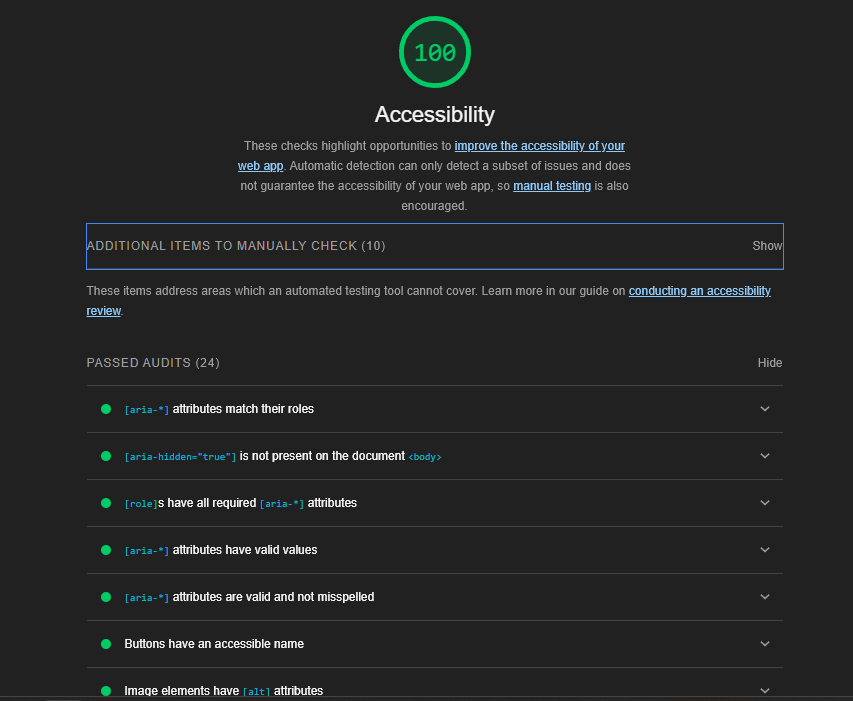
\includegraphics[width=1\textwidth]{attachments/testy-dostepnosci}
    \caption{Widok testu dostępności dla naszej aplikacji}
    \label{fig:testy-dostepnosci}
    \end{figure}


	%! Author = Wiktor Rostkowski
%! Date = 29/04/2024

\chapter{Testy}
\label{ch:testy}

%! Author = Wiktor Rostkowski, Mateusz Budzisz
%! Date = 29/04/2024

\chapter{Testy}
\label{ch:testy}

\section{Testy jednostkowe}
\label{sec:testy-jednostkowe}
W ramach projektu potok frontend wykonał 151 testów. \newline
W ramach projektu potok backend wykonał 159 testów. \newline
W ramach projektu potok dokumentacja wykonał 328 testów. \newline

\section{Testy wydajnościowe}
\label{sec:testy-wydajnosciowe}
Lighthouse
\section{Testy funkcjonalne}
\label{sec:testy-funkcjonalne}

\begin{figure}[H]
    \centering
    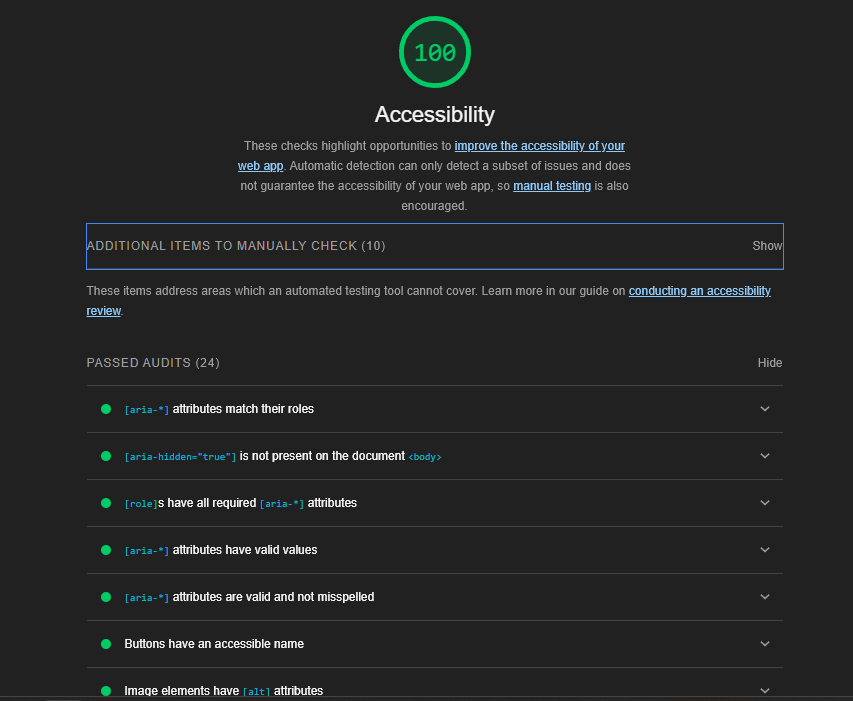
\includegraphics[width=1\textwidth]{attachments/testy-dostepnosci}
    \caption{Widok testu dostępności dla naszej aplikacji}
    \label{fig:testy-dostepnosci}
    \end{figure}





	% Początek słownika, akronimów i bibliografii
	\printbibliography[heading=bibintoc]
	\printglossary[type=\acronymtype]
	\printglossary
	% Koniec słownika, akronimów i bibliografii

\end{document}
